\chapter{The Pipeline}
\label{sec:pipeline}

\ifpdf
    \graphicspath{{5_pipeline/figures/PNG/}{5_pipeline/figures/PDF/}{5_pipeline/figures/}}
\else
    \graphicspath{{5_pipeline/figures/EPS/}{5_pipeline/figures/}}
\fi

The design goal of the pipeline is to accept timeslices as input and output a \texttt{0} or \texttt{1} indicating whether they need to be discarded or saved respectively. Two classes were identified: \texttt{class\_0} comprised timeslices with just noise and \texttt{class\_1} included timeslices with event and noise hits. Henceforth, the thesis refers to \texttt{class\_1} timeslices as event timeslices, but they contain both noise and event hits.

Stakeholder knowledge and data exploration (Chapter \ref{sec:exploration}) identified 6 key variables - \texttt{pos\_x, pos\_y, pos\_z, time, group} (timeslice) and \texttt{label}. Since neutrinos are identified by both spatial and time differences between each other, an ideal dataset would contain all four variables \cite{km3net_2017}. However, generating a 4D mesh with \texttt{time} was not feasible, as the process is complicated and relatively under-developed \cite{otomo2014direct}. Instead, \texttt{time} was combined with spatial coordinates to create three permutations of the dataset - (\texttt{x, y, time}), (\texttt{x, z, time}) and (\texttt{y, z, time}). The following chapter discusses each component of the pipeline in detail. All three datasets were processed and transformed in the same manner, so details described in the following pipeline are applicable to all three datasets.

\section{Generation of Point Clouds}
The first step in the pipeline was to build 3D point clouds for each timeslice and save them as \texttt{.xyz} files. In order to do so, a few preliminary steps were undertaken. First, timeslices were divided into two classes whereby one contained only noise and the other contained both noise and event hits. Most timeslices with only noise had an average of 6500 hits per timeslice, but there were a few timeslices that had a single noise hit. Likewise, timeslices with event hits had an average of 6900 hits per timeslices, but some timeslices had only 3 event hits. Discussion with domain scientists indicated that such groups represented an unrealistic scenario. Therefore, they were excluded from the data as they would not be able to provide a quality training sample.

Figure \ref{fig:p0_countplot_ci} shows class imbalance before and after selection of the largest timeslices per class. It shows imbalance both across the noise and events class; and also within the events class. Sub-figure \ref{fig:p0_class_imbalance} shows that the noise timeslices had fewer noise hits compared to the noise hits in event timeslices. Moreover, within the event timeslices, there is significant disparity between the number of noise and event hits. Sub-figure \ref{fig:p0_class_imbalance} indicates that the class imbalance needed to be improved as it may affect training and bias the classifier towards the majority class. Further, the entire dataset was not required for training. So, in order to continue with a smaller, quality training data, the top 200 timeslices were taken for each class. For the events class, timeslices were sorted in a descending order based on the number of event hits they contained. The largest 200 of these timeslices were then selected. Similarly, the top 200 noise timeslices were also selected. 

\begin{figure}[ht!]   
\centering
\subfloat[Count of Noise and Event Hits from All Timeslices]{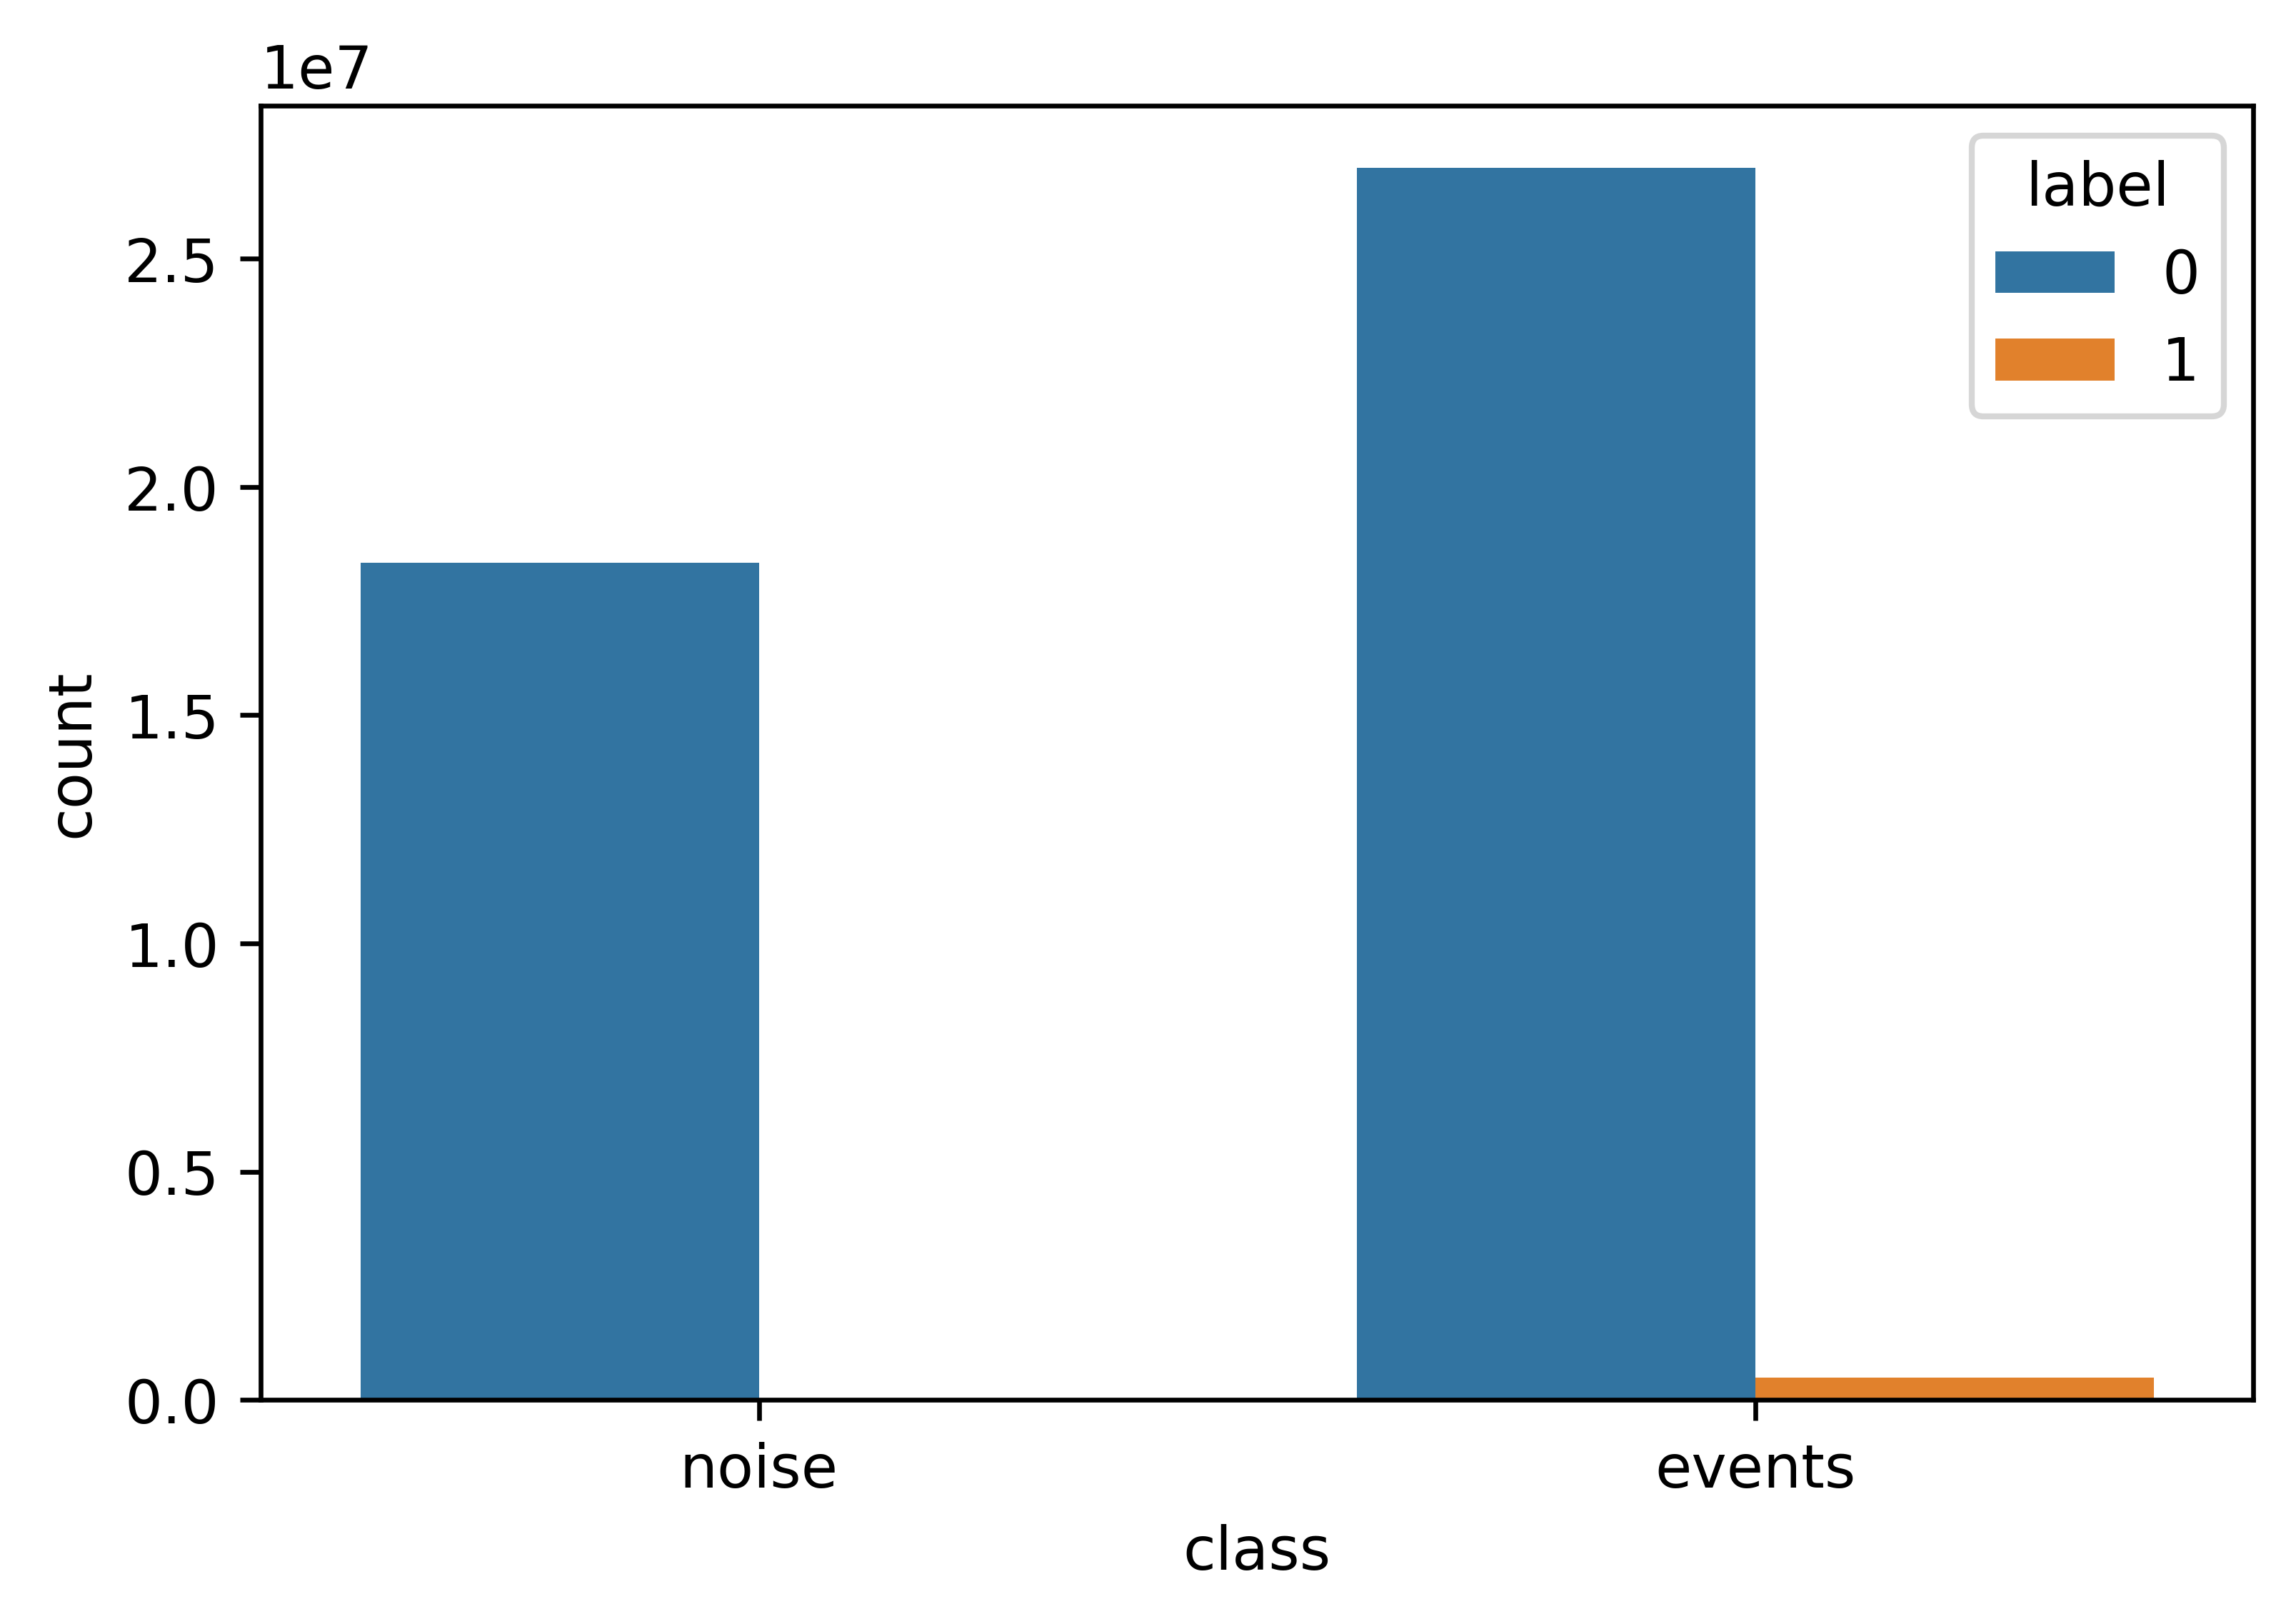
\includegraphics[width=0.48\textwidth, keepaspectratio]{class_imbalance}\label{fig:p0_class_imbalance}}
\subfloat[Count of Noise and Event Hits for 200 Noise and Event Timeslices]{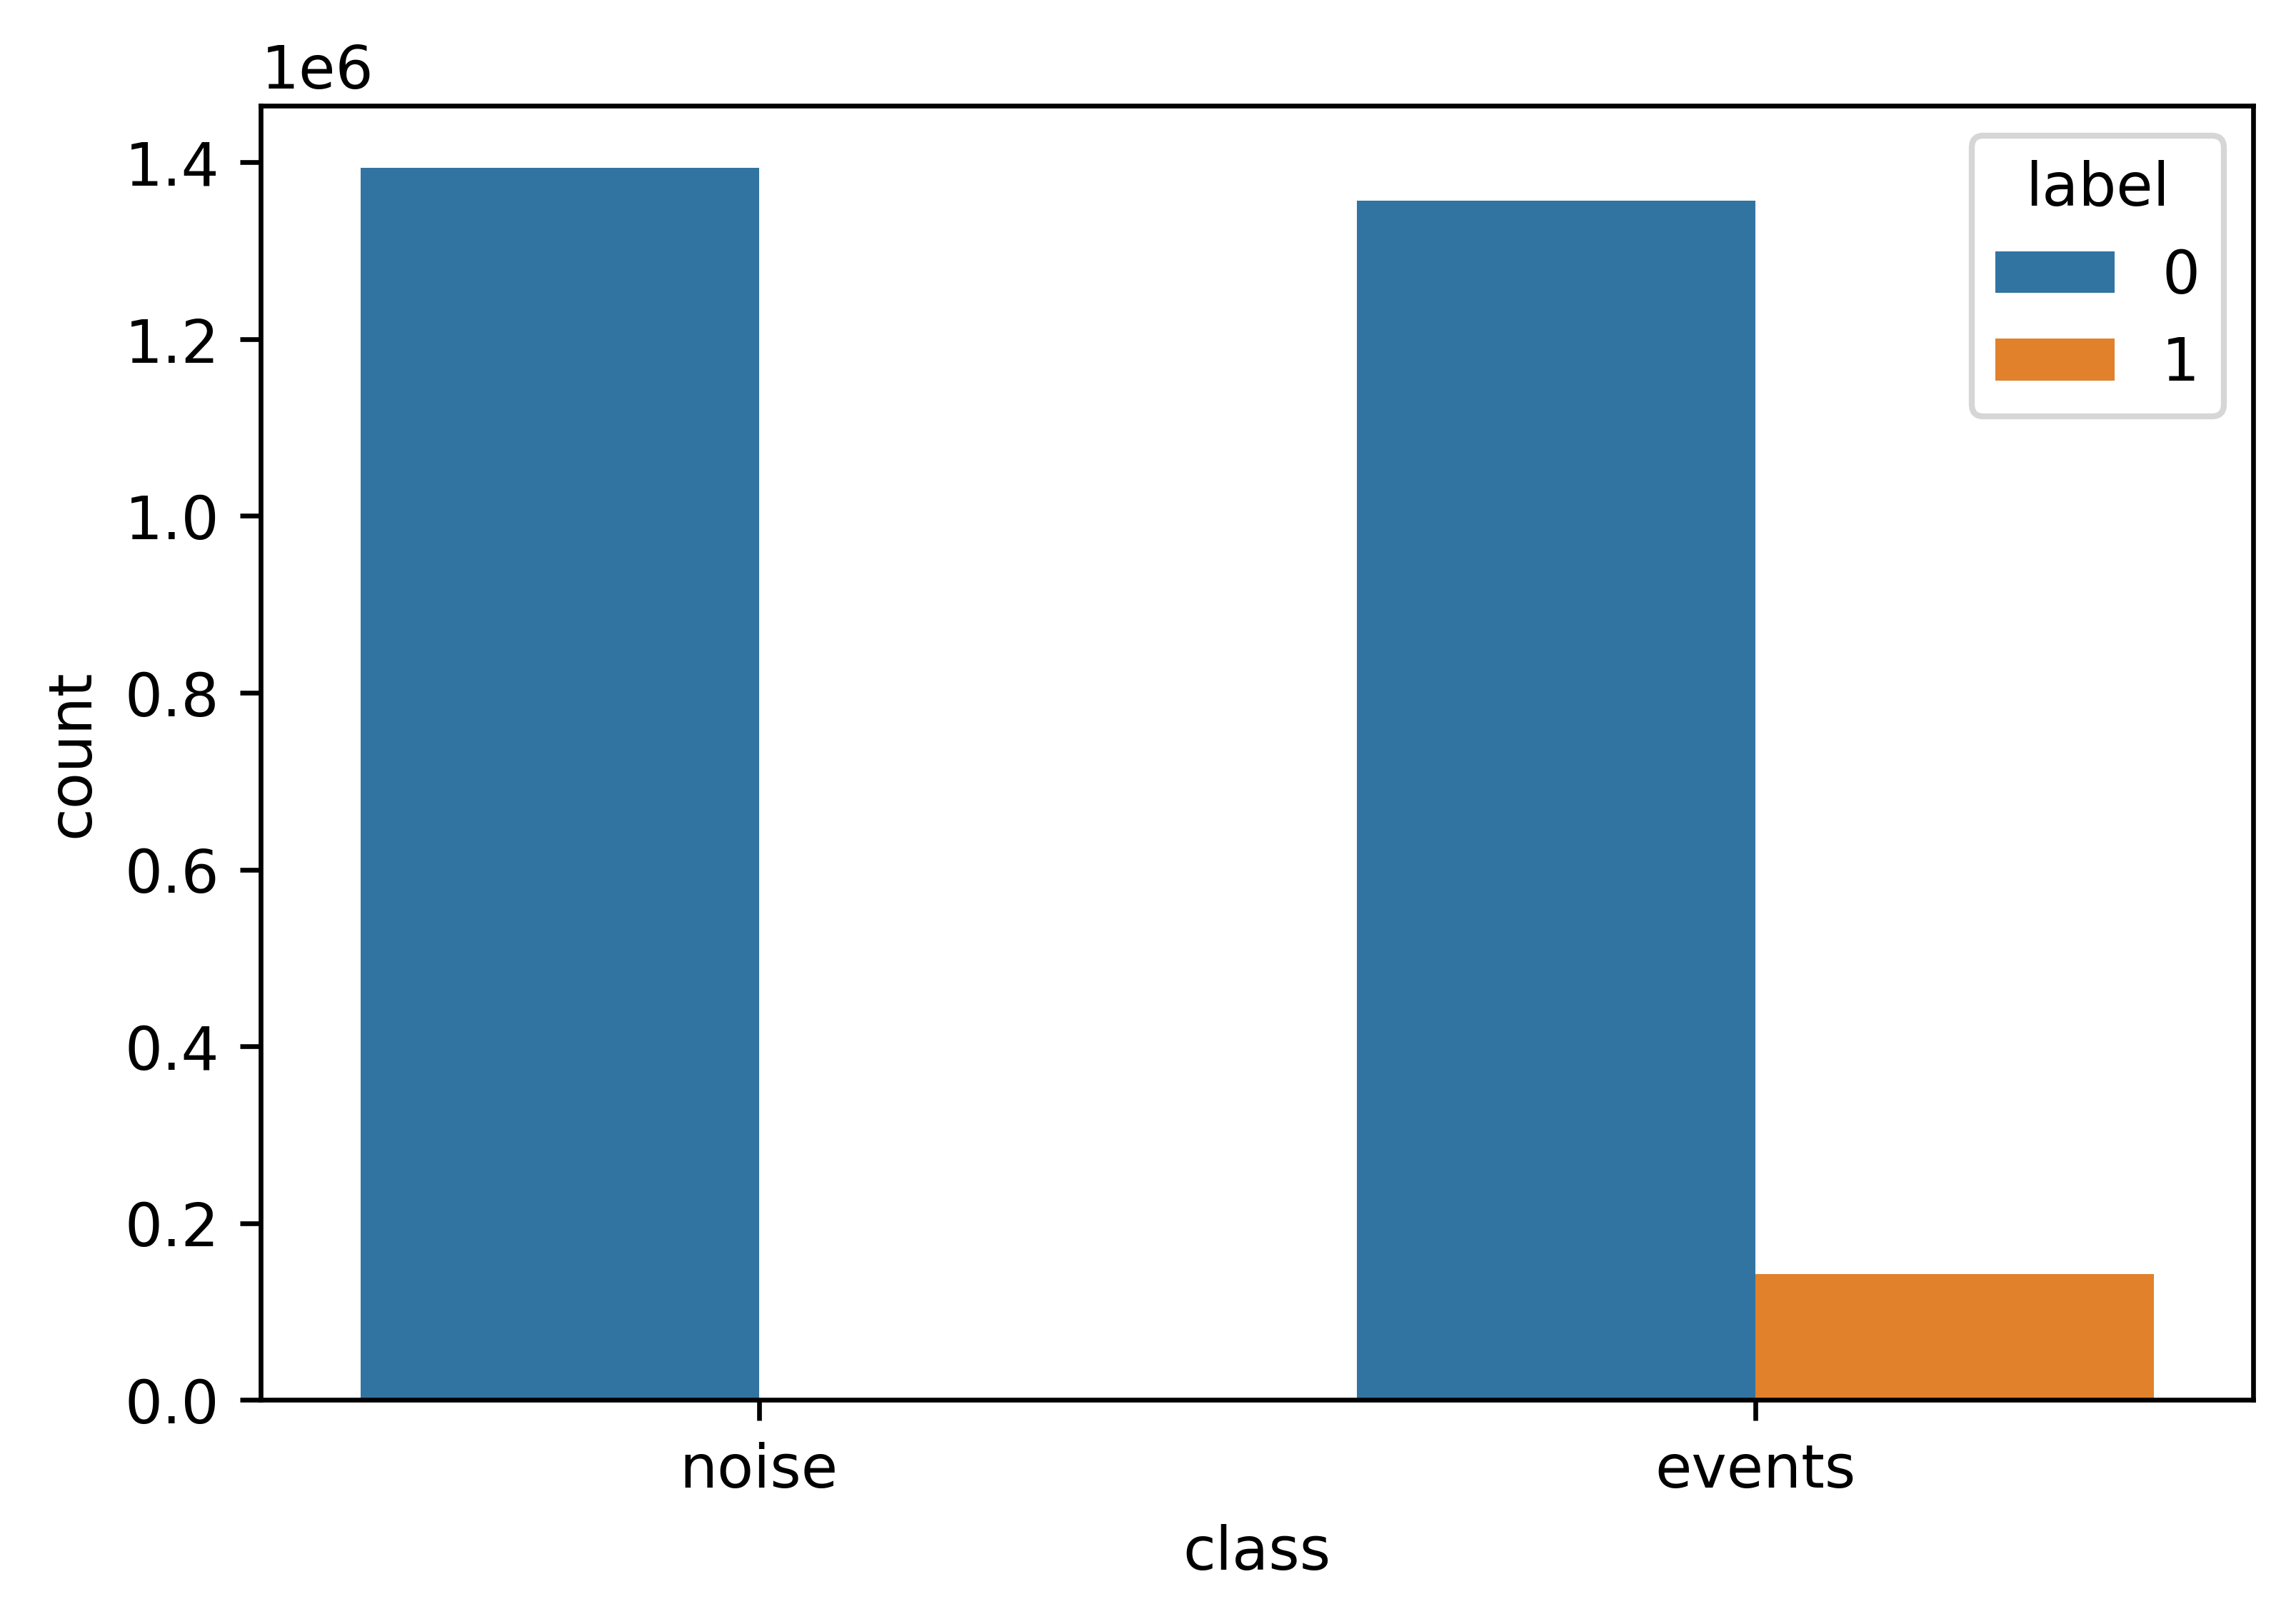
\includegraphics[width=0.48\textwidth, keepaspectratio]{class_imbalance_after_sampling}\label{fig:p0_200_class_imbalance}}
\caption[]{Class Imbalance Before and After Selection of Top 200 Timeslices Per Class}
\label{fig:p0_countplot_ci}
\end{figure}

Sub-figure \ref{fig:p0_200_class_imbalance} shows the class imbalance after selecting the top timeslices. The noise hits are now equal between the two classes. Further, there is some improvement between the event and noise hits within the events class. This indicated that taking the largest timeslices helped make the dataset more uniform and balanced for training.

Data for the 200 event timeslices were further observed. It was seen that there were a total of 27,485,996 hits, of which only 489,906 were event hits. Positive hits formed only 1.78\% of the data. The maximum number of hits a timeslice was 1692 and the smallest number of hits in a timeslice was 487. On average, timeslices had around 700 event hits. In contrast, these timeslices had 7000 noise hits on average. All timeslices were saved as point clouds under their respective classes - \texttt{class\_0} comprising of noise point clouds and \texttt{class\_1} comprising of event and noise point clouds.


\section{Feature Engineering}
Feature engineering is the process through which data can be transformed in a manner that either brings new information to light or provides more structure to the data, making learning easier for the network \cite{guyon2003introduction}. Feature engineering was included in the pipeline due to three main reasons.Visual data exploration (Section \ref{sec:exploration}) revealed unrelated variables with no significant patterns. Next, visual inspection of both point clouds and their corresponding 3D meshes showed lack of potential structure. Finally, preliminary results from training on data without feature engineering showed the need for additional information (Appendix \ref{appendix}).

\begin{figure}[ht!]
    \centering 
    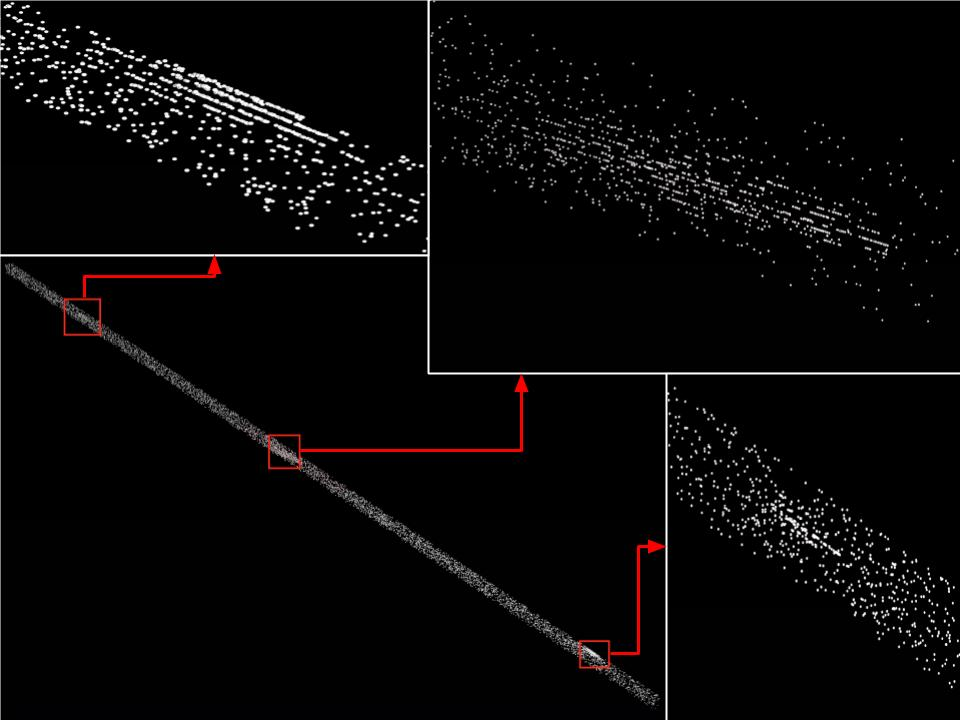
\includegraphics[width=\textwidth, height=10cm]{g_615.jpg}
    \caption{Point Cloud of the Largest Event Timeslice}
    \label{fig:g_615}
\end{figure}


Figure \ref{fig:g_615} shows a timeslice that contained the highest number of event hits. The point cloud has three event regions highlighted in red that are very hard to identify. These regions were visualised under a highly zoomed perspective using MeshLab \footnote{https://www.meshlab.net/\#description} and shows very minimal differences between event hits and the surrounding noise \cite{LocalChapterEvents:ItalChap:ItalianChapConf2008:129-136}. Figure \ref{fig:g_0} on the other hand shows a point cloud of the timeslice with the highest number of noise. Based on the observed point clouds, it was decided that the data could be enhanced by elimination of points. Certain noise hits could be identified as outliers and removed in order for clusters of event hits to stand out more. 

\begin{figure}[ht!]
    \centering 
    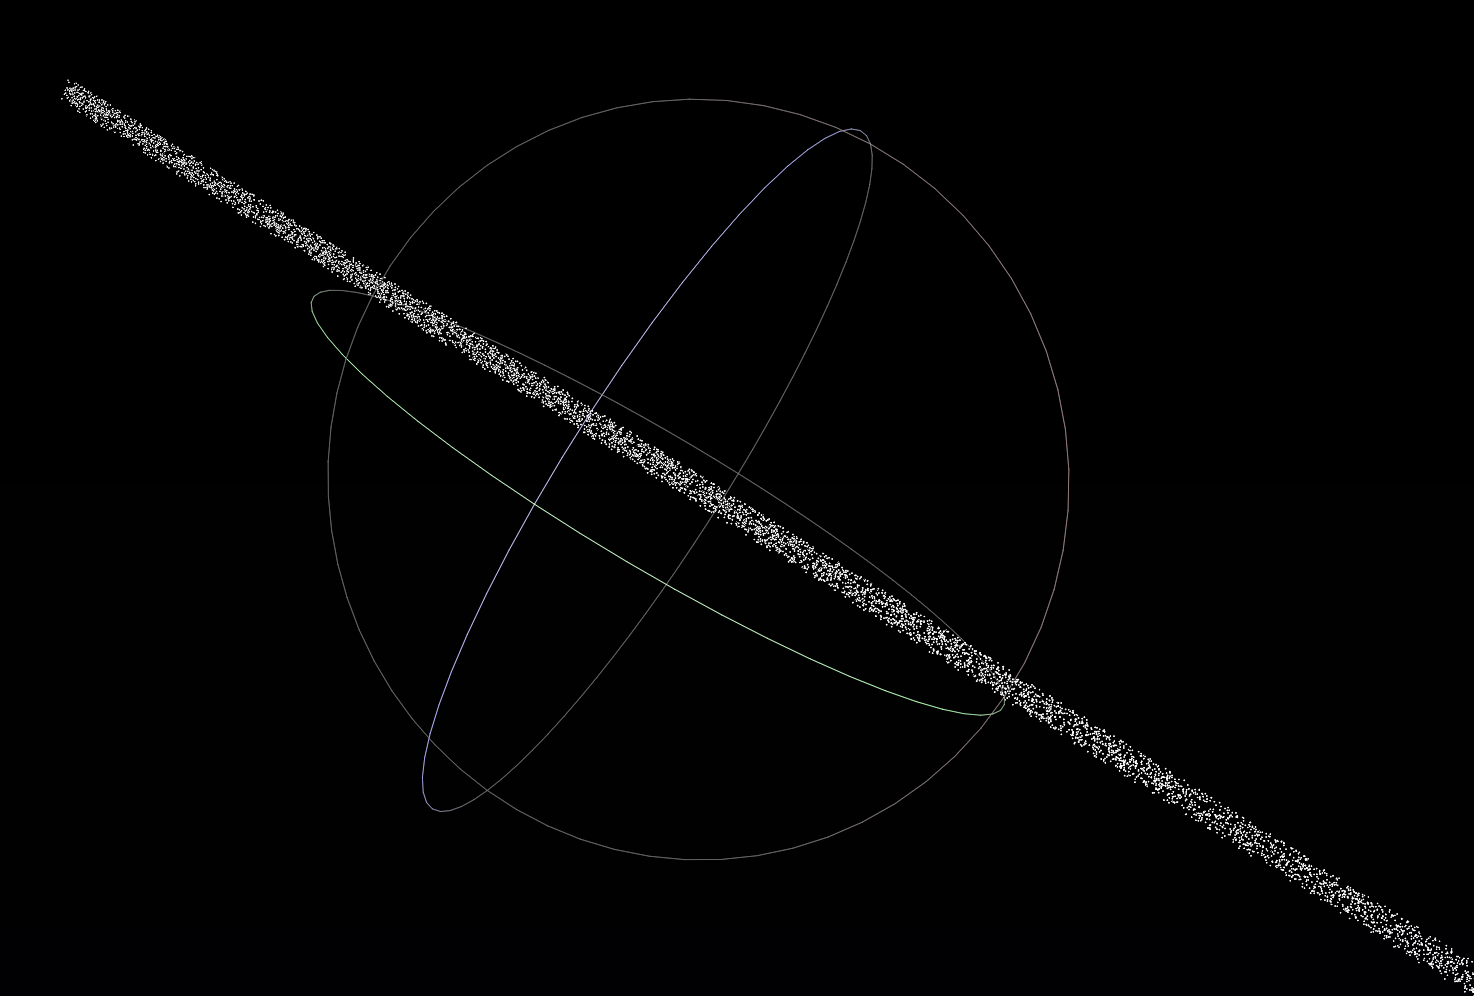
\includegraphics[width=\textwidth, height=6cm]{group_0.png}
    \caption{Point Cloud of the Largest Noise Timeslice}
    \label{fig:g_0}
\end{figure}

Removing outliers from point clouds are a common task and often manually removed using point cloud processing software \cite{LocalChapterEvents:ItalChap:ItalianChapConf2008:129-136}. Surface fitting-based methods are a popular means of outlier removal. Here, a triangulated surface gets generated and criterion such as Moving Least Squares with Lagrangian operators are used to identify "rough" features from irregular regions \cite{lipman2007parameterization}. Discontinuous operators-based method is another reliable technique whereby regions of points are detected using density depth maps and removed based on visibility conflict \cite{qi2016hedged}. All methods described have the advantage of being conceptually accurate \cite{ning2018efficient}. Discontinuous operators based methods however work only on specific outliers and are inapplicable elsewhere \cite{qi2016hedged}. Surface based methods can work well on logical shapes but may not make sense for irregular, unknown shapes. They can also be very time consuming due to the typically large size of point clouds \cite{lipman2007parameterization, kobbelt2004survey}. This thesis required a technique that could work well on irregular point clouds. Moreover, the focus was on providing fast processing, rather than precise outlier detection. This is because the transformed point clouds would ultimately be passed onto PointNet that should perform additional computations to differentiate between the two classes. Based on these requirements, a simple radius-based outlier detection method was finalised \cite{ning2018efficient}. 

\begin{figure}[ht!]
    \centering 
    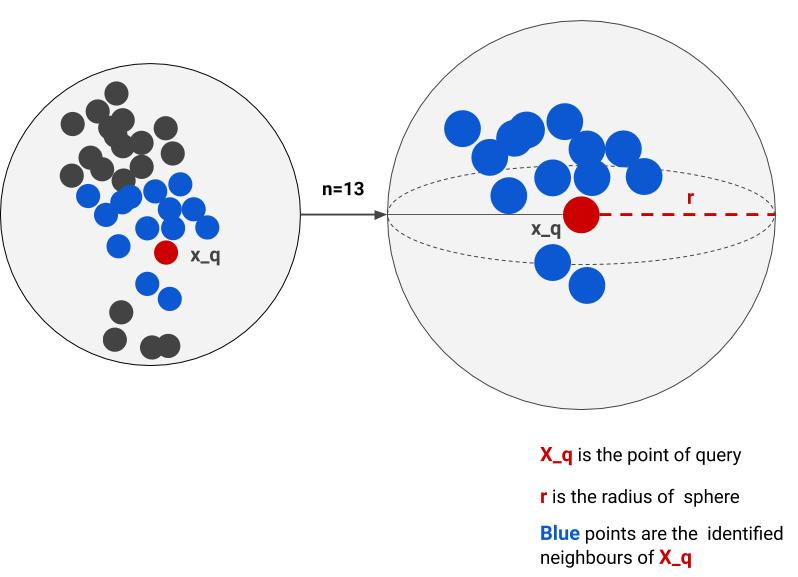
\includegraphics[width=0.7\textwidth,height=6cm, keepaspectratio]{p1_rbof.jpg}
    \caption{Demonstration of the Principle of Radius-Based Outlier Removal on A Set of Points}
    \label{fig:p1_rbof}
\end{figure} 

The principle of radius-based outlier filter (RBOF) is that if the number of points in the sphere of radius \texttt{r} centred at the query point \texttt{X\_q} is lower than a threshold \texttt{n}, then \texttt{X\_q} will be marked as an outlier and removed \cite{li2019overlapping}. Figure \ref{fig:p1_rbof} explains the concept of radius-based outlier removal where the red point (\texttt{X\_q}) is the point of interest. The number of neighbours is specified to be 13. Based on a specified radius \texttt{r}, there are 13 blue points that lie within the sphere of \texttt{X\_q}. Thus, \texttt{X\_q} is identified as outlier. Visual analysis of point clouds such as in Figures \ref{fig:g_615} and \ref{fig:g_0} helped determine that noise timeslices had roughly evenly spaced points. Therefore, the goal of RBOF was that fewer outliers would be detected and removed. Event timeslices however showed clustering of points, so here, the algorithm would detect and remove more outliers, especially the noise hits around the event clusters. 

% Feature Engineering process
\begin{figure}[ht!]
    \centering 
    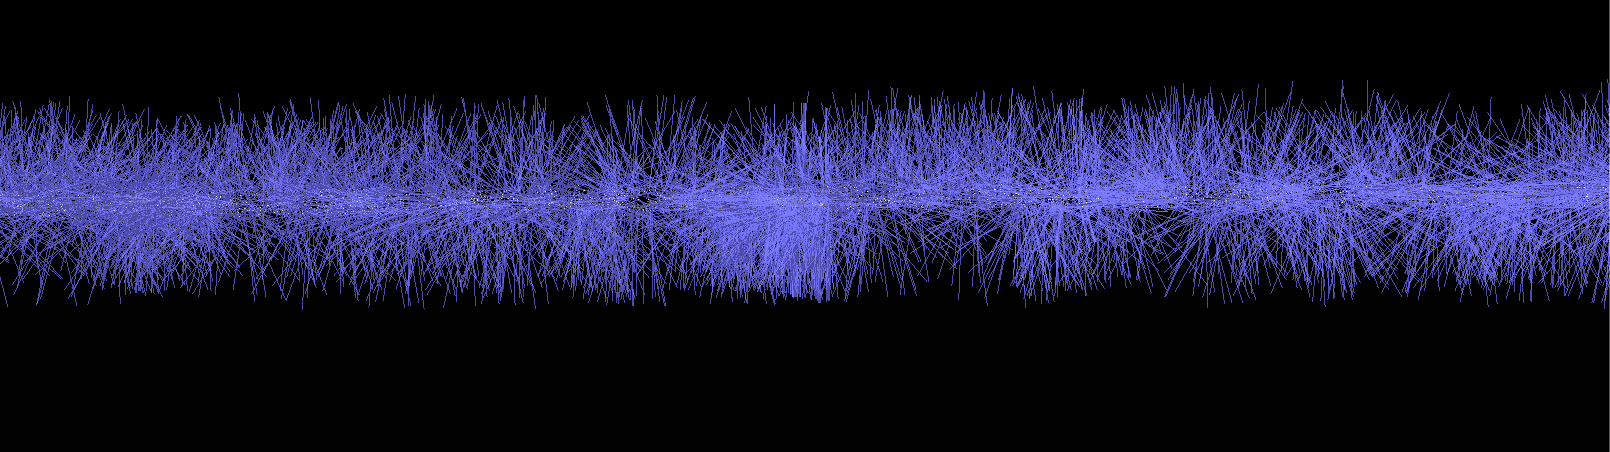
\includegraphics[width=\textwidth, height=4cm,keepaspectratio]{p1_normals_10.png}
    \caption{Normals computed for a Timeslice with Nearest Neighbours Specified as 10}
    \label{fig:p1_normals_10}
\end{figure}

Open3D\footnote{http://www.open3d.org/} was used to identify outliers and perform feature engineering. First, all \texttt{.xyz} files from each class were transformed from an array of 3D coordinates to an \texttt{o3d.geometry.PointCloud} geometry. Next, normals were computed for each point because surface reconstruction based 3D meshing requires normals of the point cloud \cite{mitra2003estimating}. The number of neighbours used to estimate normals was set to \texttt{300}, due to the large number of points per point cloud. 


Figure \ref{fig:p1_normals_10} shows the normals for a timeslice with the largest number of event hits, when computed with the default \texttt{10} neighbours. The purple markers indicate the direction of the normal. Ideally, the markers for all points must face in the same direction, which is not the case in Figure \ref{fig:p1_normals_10}. Figure \ref{fig:p1_normals} shows the same timeslice, recomputed with \texttt{300} nearest neighbours. The markers now approximately point in the same direction. The highlighted regions in the figure correspond to event hits and show interesting behaviour. The normals computed at these locations all point at different directions. 

\begin{figure}[ht!]
    \centering 
    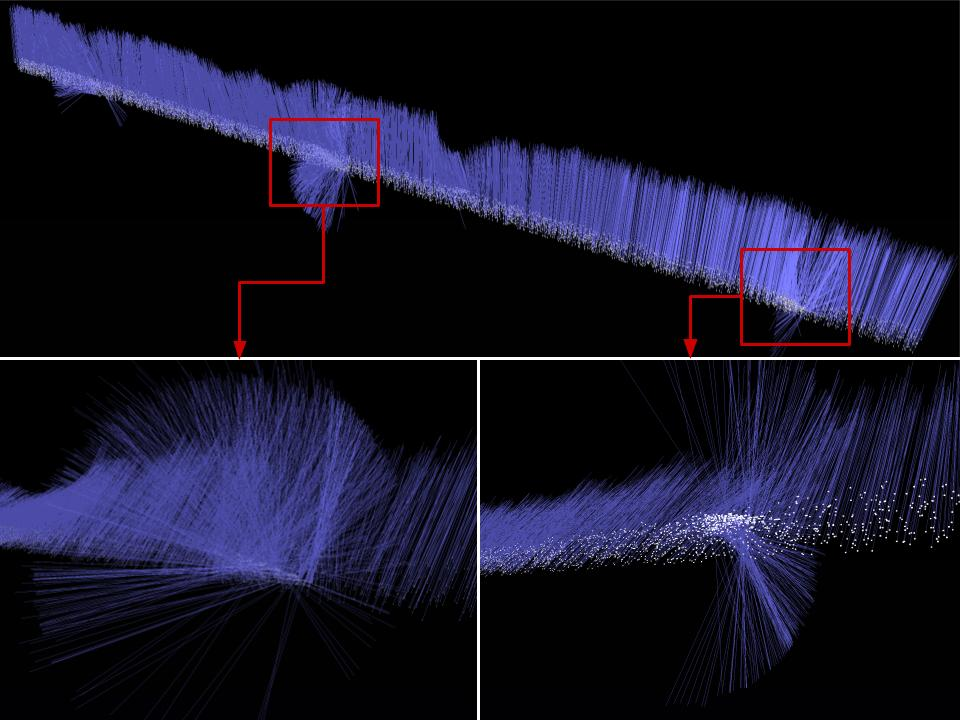
\includegraphics[width=\textwidth,keepaspectratio]{p1_normals.jpg}
    \caption{Normals computed for a Timeslice with Nearest Neighbours Specified as 300}
    \label{fig:p1_normals}
\end{figure}

With the point clouds normalised, the radius-based outlier detection was finally performed. The minimum amount of points that the sphere should contain (\texttt{nb\_points}) was left as the default value of \texttt{32} neighbours. The \texttt{radius} of the sphere that would be used for counting the neighbours was set to vary for each point cloud because of their irregular shapes and densities. A fixed radius value would not generalise well and produce inaccurate results. In order to identify a suitable radius, the nearest neighbour algorithm was used to compute the distance from a point to its nearest neighbour in the point cloud \cite{cui2018flexible}. Once an array of all the distances were obtained, they were averaged and multiplied by a factor of 3.6 to account for scaling \cite{zhou2018open3d}.

\begin{figure} [ht!]
    \centering
    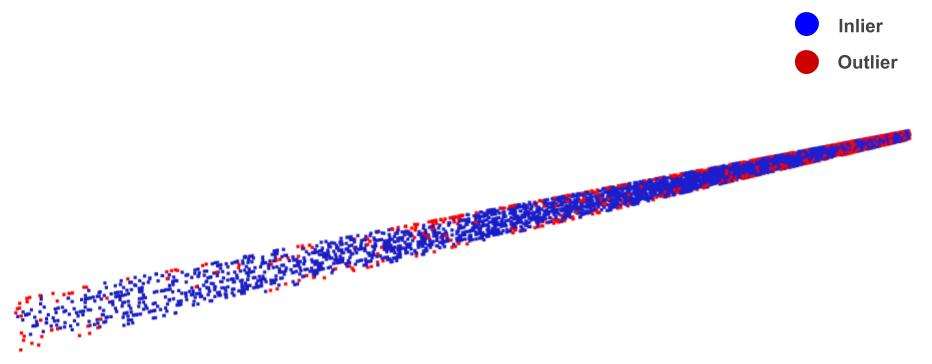
\includegraphics[width=0.7\textwidth, height=4cm]{p1_outlier_noise}
    \caption{Result of Radius-Based Outlier Detection on Timeslice with Only Noise}
    \label{fig:p1_outlier_noise}
\end{figure}

Figure \ref{fig:p1_outlier_noise} shows the result of applying the outlier removal on a timeslice with only noise. The algorithm identified inliers in blue and outliers in red. 

\begin{figure}[htb!]   
\centering
\subfloat[Noise Timeslice Before and After Outlier Removal]{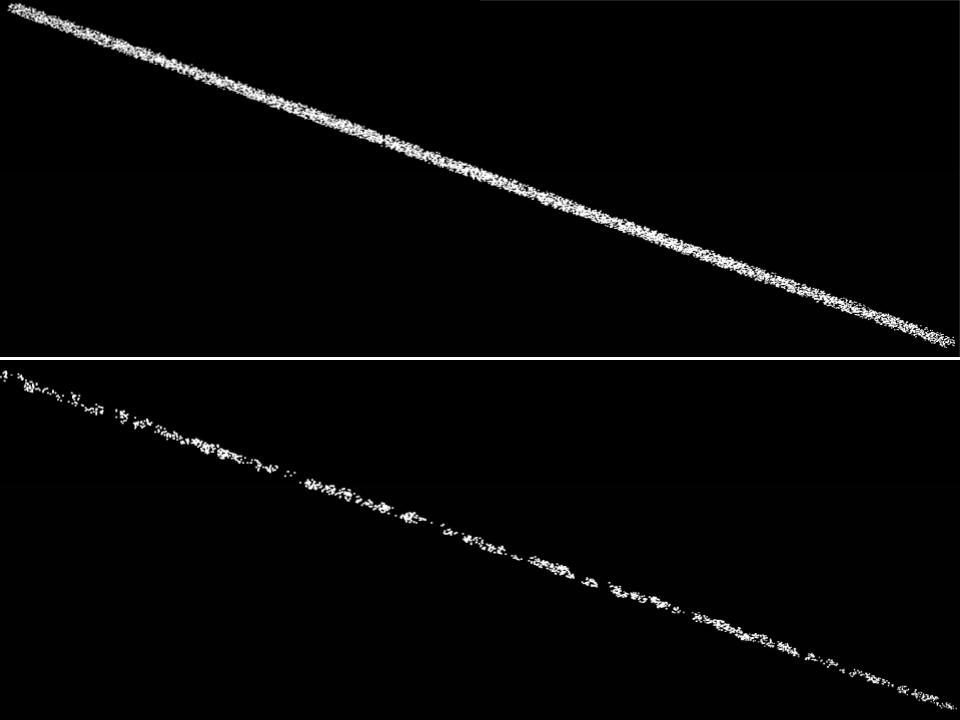
\includegraphics[width=0.49\textwidth,height=5cm]{p1_noise_after_outlier_removal.jpg}\label{fig:p1_noise_after_outlier}}
\hspace{0.1cm}
\subfloat[Event Hits Timeslice Before (Top) and After (Bottom) Outlier Removal]{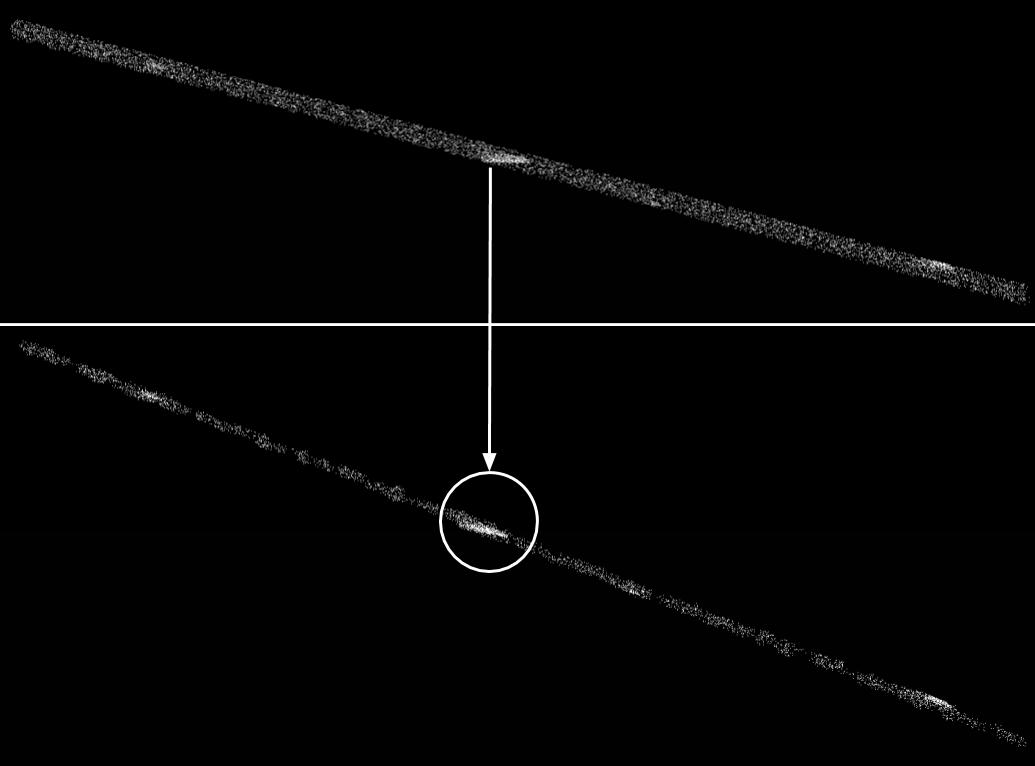
\includegraphics[width=0.49\textwidth,height=5cm, keepaspectratio]{p1_hits_after_outlier_removal.jpg}\label{fig:p1_hits_after_outlier}}
\caption[]{Noise and Event Hits Timeslices Before (Top) and After (Bottom) Radius-Based Outlier Detection}
\label{fig:before_after_outlier}
\end{figure}

Figure \ref{fig:before_after_outlier} shows an example of a noise and event hits timeslices both before and after removal of outliers. As expected, the RBOF found a higher incidence of outliers in the event timeslice. The resulting point cloud is more simplified with the event hit clusters intact, as highlighted in Figure \ref{fig:p1_hits_after_outlier}. Similarly, Figures \ref{fig:p1_outlier_615} and \ref{fig:p1_outlier_hit} shows the result of the algorithm on timeslices with event hits. As expected, event timeslices show higher number of outliers due to the presence of event clusters.

\begin{figure}[htb!]   
\centering
\subfloat[Timeslice with Highest Event Hits]{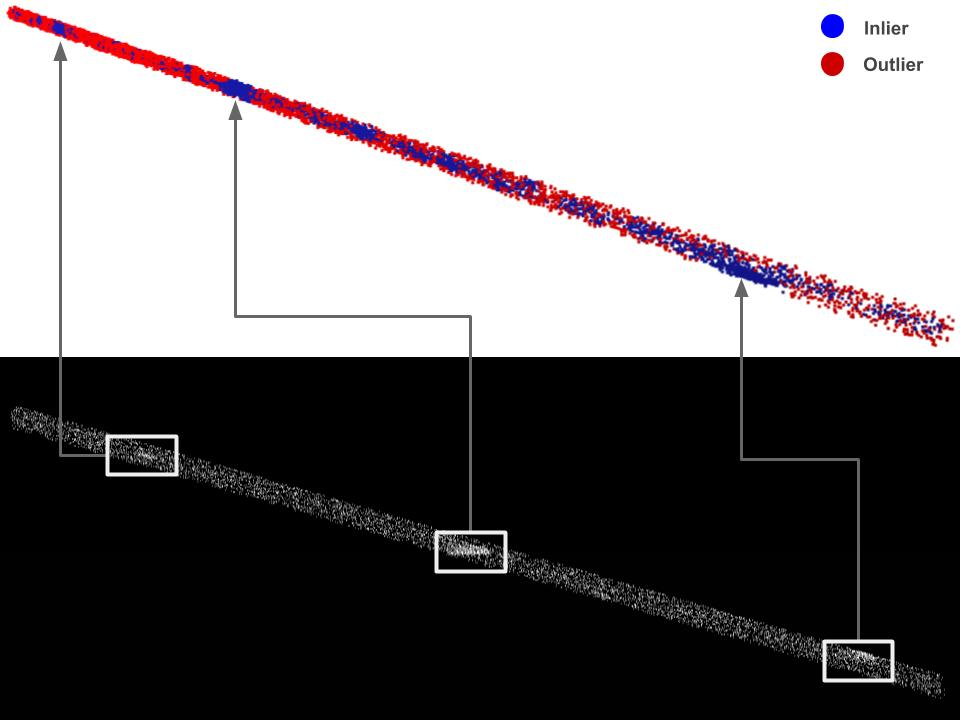
\includegraphics[width=\textwidth,keepaspectratio]{p1_outlier_615}\label{fig:p1_outlier_615}}

\subfloat[Another Event Hits Timeslice]{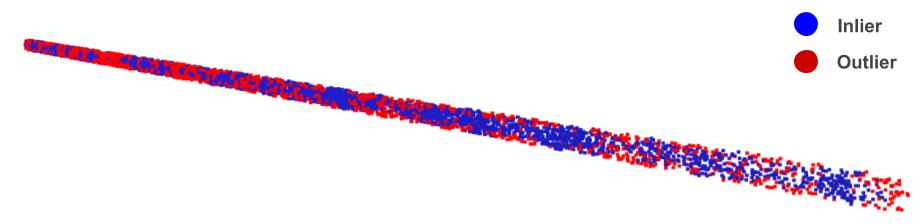
\includegraphics[width=\textwidth, height=3cm]{p1_outlier_hit}\label{fig:p1_outlier_hit}}
\caption[]{Result of Radius-Based Outlier Detection On Different Event Timeslices}
\label{fig:p1_outlier_removal}
\end{figure}

\section{3D Mesh Generation}
With the feature engineering completed, \texttt{.xyz} files were converted to 3D meshes. Meshes are a collection of geometric properties - vertices, faces and edges that describe a 3D object \cite{kim2006complete}. There are several algorithms that can convert 3D coordinates to meshes but two of the most popular algorithms were considered and evaluated \cite{kim2006complete}.

\textbf{Ball Pivoting Algorithm (BPA)} ``rolls" a virtual ball across the point cloud ``surface". It forms a triangle from the three nearest points and then rolls along that triangle to another set of three points where it forms a new triangle \cite{bernardini1999ball}. In this manner, the algorithm continues until all points are converted to a mesh. BPA requires the radius of the ball to be specified such that it is slightly larger than the average space between points \cite{bernardini1999ball}. For this thesis, using an average radius value would cause problems in the event hit clusters as the distance between points in those regions may be less than the size of the ball. This would lead the ball to roll over those points and ignore them. Given the irregular, unknown symmetry with sets of close points in event clusters, it was likely that BPA would miss the details that could indicate presence of event hits. 

\begin{figure}[ht!]   
\centering
\subfloat[Event Timeslice: Highlighted Area Corresponds to Event Hits Cluster]{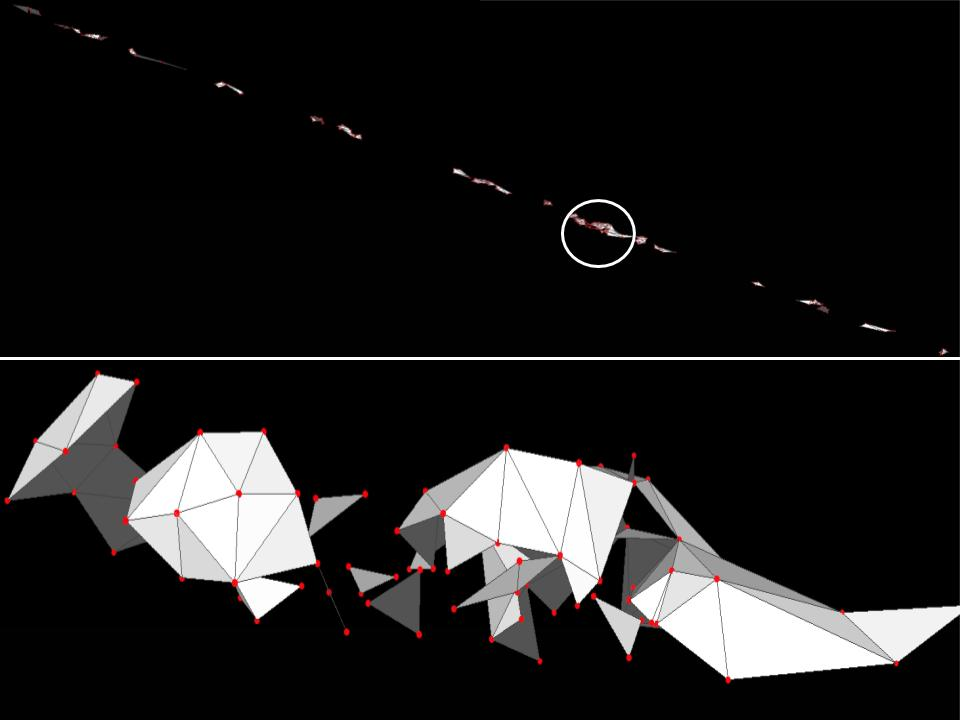
\includegraphics[width=0.49\textwidth, keepaspectratio]{p2_hits_bpa}\label{fig:p2_hits_bpa}}
\hspace{0.01cm}
\subfloat[Noise Timeslice]{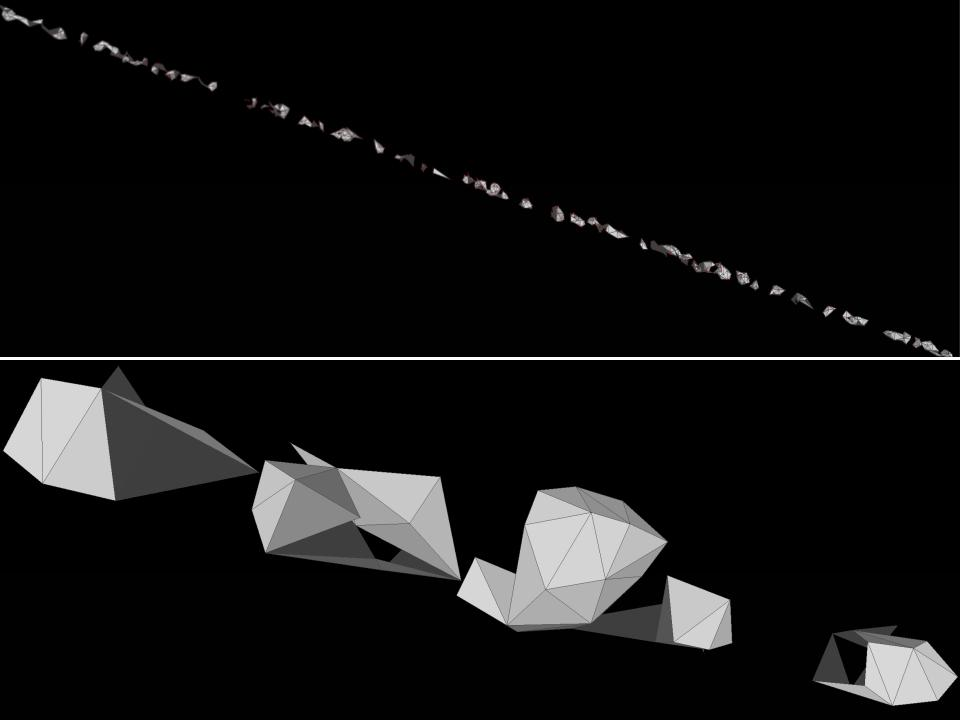
\includegraphics[width=0.49\textwidth, keepaspectratio]{p2_noise_bpa}\label{fig:p2_noise_bpa}}
\caption[]{Noise and Event Timeslices After Applying Ball Pivoting Algorithm}
\label{fig:p2_bpa}
\end{figure}

Figure \ref{fig:p2_bpa} shows the transformed point clouds after applying BPA. Figure \ref{fig:p2_hits_bpa} shows an events timeslice where event hits (in red) are overlaid with the corresponding 3D mesh for comparison. The region in focus shows an event cluster. The algorithm rolled over and missed several points, leaving gaps in the mesh. On the other hand, Figure \ref{fig:p2_noise_bpa} shows the effect of BPA on a noise timeslice. Due to the generally evenly spaced nature of noise, the algorithm was able to capture most points. However, the two meshes don't show significant differences between each other since the event clusters are not particularly enhanced. It indicated that BPA would not be sufficient for the PointNet to learn. 


% \Poisson
\textbf{Poisson Surface Reconstruction} is an implicit meshing algorithm by Kazhdan et al. (2006) that envelops points in a smooth "cloth". It tries to fit a surface from the original point set by creating an entirely new point set representing an iso-surface linked to the normals \cite{kazhdan2006poisson}. As it tries to create a watertight surface, it seemed a more promising solution for the detailed event regions. Poisson Surface Reconstruction required several parameters for the octree that is used for the reconstruction \cite{kazhdan2006poisson} - depth, scale and fit. The octree \textit{depth} specifies the level of detail of re-construction and is the most significant parameter. The \textit{scale} describes the ratio between the diameter of the cube used for reconstruction and the diameter of the samples’ bounding cube. \textit{fit} lets the re-constructor use linear or non-linear interpolation to estimate the positions of iso-vertices \cite{kazhdan2006poisson}.

\begin{figure}[ht!]   
\centering
\subfloat[Event Timeslice: Highlighted Area Corresponds to Event Hits Cluster]{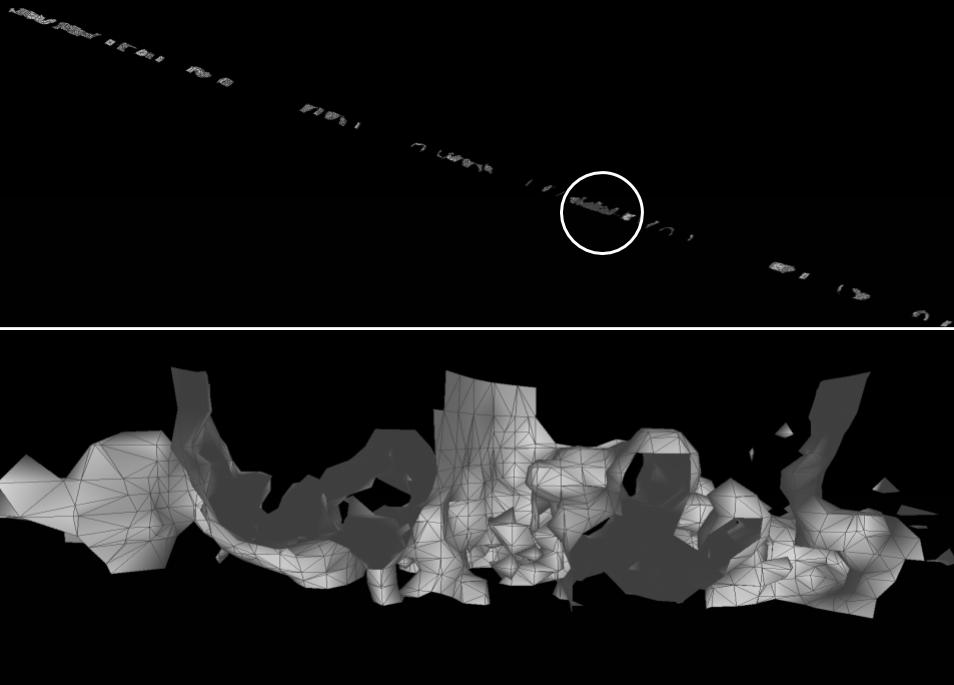
\includegraphics[width=0.49\textwidth, keepaspectratio]{p2_hits_sp}\label{fig:p2_hits_sp}}
\hspace{0.01cm}
\subfloat[Noise Timeslice: Highlighted Area Corresponds to Noisy Artefact ]{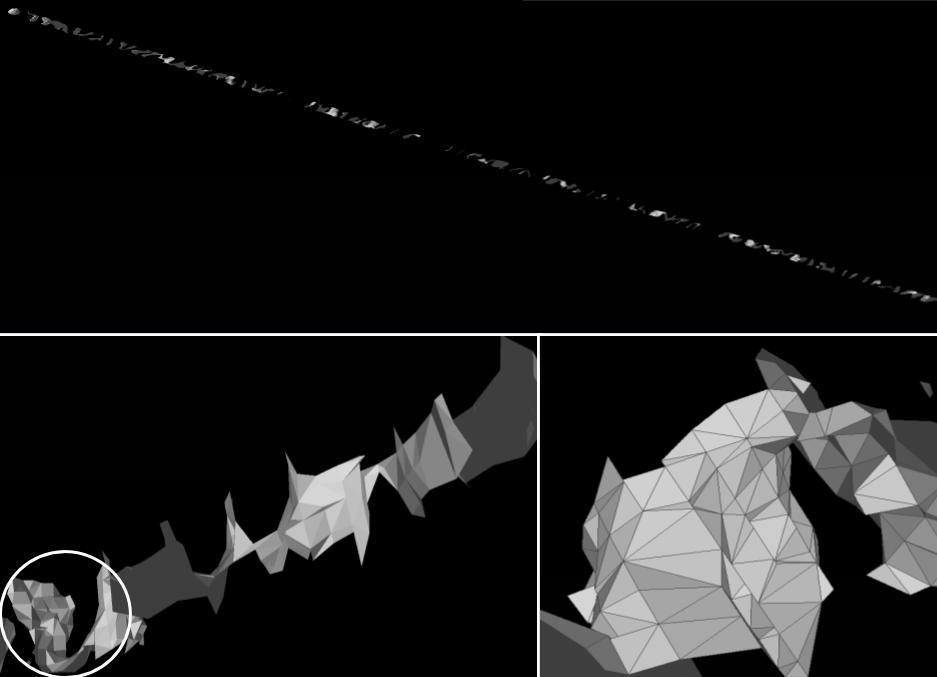
\includegraphics[width=0.49\textwidth, keepaspectratio]{p2_noise_sp}\label{fig:p2_noise_sp}}
\caption[]{Noise and Event Timeslices After Applying Surface Poisson Reconstruction}
\label{fig:p2_sp}
\end{figure}

Default parameters of depth \texttt{10}, octree scale \texttt{1.1} and \texttt{non-linear} interpolation were used  \cite{LocalChapterEvents:ItalChap:ItalianChapConf2008:129-136}. Figure \ref{fig:p2_sp} shows the same timeslices as before, rendered with Poisson Surface Reconstruction. Poisson Surface Reconstruction shows a more detailed mesh for the event hits region in the event timeslice in Figure \ref{fig:p2_hits_sp}. Figure \ref{fig:p2_noise_sp} shows the algorithm rendered on the noise timeslice. The surface is more or less flat and even. However, the Reconstruction algorithm produced some noisy artefacts, as highlighted in the image.

Based on the difference in mesh detail between BPA and Poisson Surface Reconstruction, Poisson Surface Reconstruction did a better job of capturing event hits. The noisy artefacts generated in noise timeslices could pose a problem, however PointNet should be able to better distinguish between the two classes based on other features. 


\section{PointNet}
PointNet was implemented in PyTorch \footnote{https://pytorch.org/} and a few modifications were made to work with the KM3NeT Data. Input batch (training examples) for PointNet can be 1D or 2D convolutions \cite{qi2017pointnet}. A convolution involves the application of a filter to the input that results in an activation function \cite{goodfellow2016convolutional}. For the thesis, 1D convolutions were used as it can help reduce dimensions and computational costs \cite{lin2013network}. In this case, the 1D convolution was the Multi-Layer Perceptron (MLP) with shared weights and kernel of size 1.

Pooling layers allow for down-sampling feature maps by means of a summary \cite{goodfellow2016convolutional}. Two common pooling methods include max pooling which summarises the most activated presence of a feature; and average pooling which summarises the average presence of a feature \cite{goodfellow2016convolutional}. Instead of using a global max pool function suggested in the paper by Qi et al. (2017), an average pool function was applied to the transformed features \cite{qi2017pointnet}. This was done because max pool was found to cause some overfitting to the KM3NeT data.

The paper by Qi et al. (2017), used Cross Entropy Loss, a typical loss function for classification \cite{qi2017pointnet}. However, thesis experiments showed that the network learned better with the negative log-likelihood (NLL) loss. As the NLL loss requires log probabilities of each class, the Log Sigmoid activation was also applied to the output layer \cite{paszke2019pytorch}. The remainder of the architecture was left unchanged. 

\subsection{PointNet Transformations}
\begin{figure}[ht!]   
\centering
\subfloat[Events Timeslice With Vertices from Mesh]{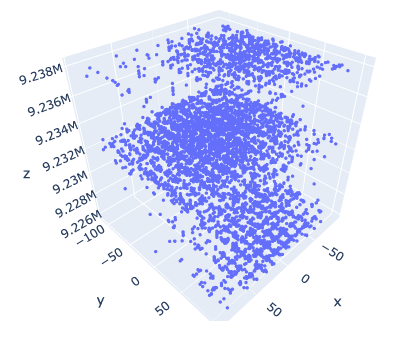
\includegraphics[width=0.49\textwidth,height=6cm,]{hits_vertices.png}\label{fig:hits_v}}
\hspace{0.01cm}
\subfloat[Noise Timeslice With Vertices from Mesh]{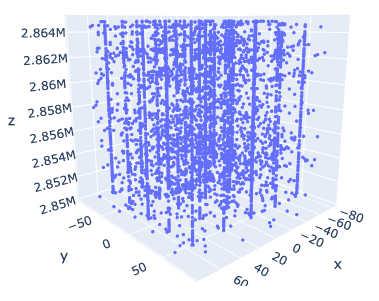
\includegraphics[width=0.49\textwidth,height=6cm]{noise_vertices.png}\label{fig:noise_v}}
\caption[]{Noise and Event Timeslices With Non-Uniform Distribution of Mesh Vertices}
\label{fig:vertices}
\end{figure}

Qi et al. (2017) stated three requirements for training point clouds with PointNet (Section \ref{sec:concepts}). Point clouds should be unordered and PointNet has to be invariant to permutations of the input set. Next, the network must be invariant to rigid transformations. Finally, the network should also capture interactions among points \cite{qi2017pointnet}. The thesis implemented the recommended transformations to the input point clouds during training and testing to ensure conformity of data to the above requirements \cite{qi2017pointnet}.

Points are not uniformly distributed across the 3D object’s surface, hindering PointNet's ability to classify them. For example, Figure \ref{fig:vertices} shows non-uniformity in the distribution of vertices from the meshes for both noise and event class. 

\begin{figure}[ht!]   
\centering
\subfloat[Event Hits Timeslice Sampled with 1024 Points]{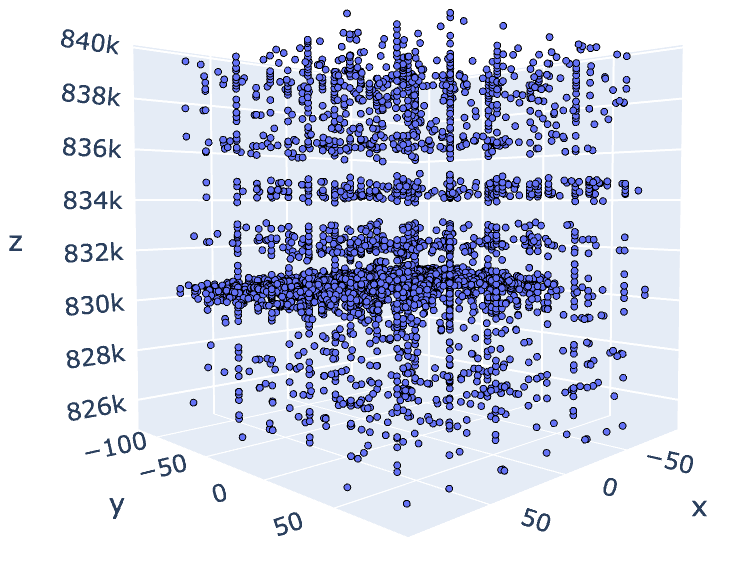
\includegraphics[width=0.49\textwidth,height=7cm, keepaspectratio]{hits_1024_sampled.png}\label{fig:hits_1024}}
\hspace{0.01cm}
\subfloat[Event Hits Timeslice Sampled with 8192 Points]{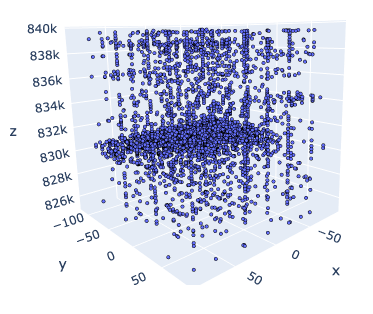
\includegraphics[width=0.49\textwidth,height=5.5cm]{hits_8192_sampled.png}\label{fig:hits_8192}}
\hspace{0.01cm}

\subfloat[Noise Timeslice Sampled with 1024 Points]{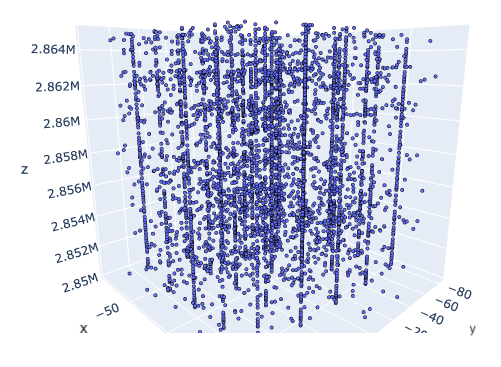
\includegraphics[width=0.49\textwidth, height=7cm, keepaspectratio]{noise_1024_sampled.png}\label{fig:noise_1024}}
\subfloat[Noise Timeslice Sampled with 8192 Points]{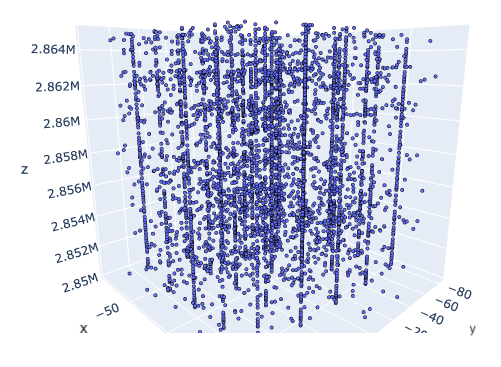
\includegraphics[width=0.49\textwidth,height=7cm, keepaspectratio]{noise_1024_sampled.png}\label{fig:noise_8192}}
\caption[]{An Example of Noise and Event Timeslices With Different Levels of Sampling}
\label{fig:sampled}
\end{figure}

PointNet also requires a fixed number of points to be sampled per point cloud \cite{qi2017pointnet}. While Qi et al. (2017) uniformly sampled 1024 points on mesh faces, it was found that this number was not sufficient for the KM3NeT Data.  Figure \ref{fig:sampled} shows both classes of point clouds randomly sampled with 1024 points and then with 8192 points (points have to be in multiples of 1024). While noise timeslices were relatively unaffected, event timeslices showed better structure with greater points. The thesis sampled one point per chosen face. Additionally, as faces had different areas, a probability was assigned to choose a particular face proportional to its area. That is, faces with higher area had higher probability of being chosen as it represented more of the surface \cite{qi2017pointnet}. In this manner, a total of 8192 point were sampled per point cloud.

\begin{figure}[ht!]   
\centering
\subfloat[Event Hits Timeslice]{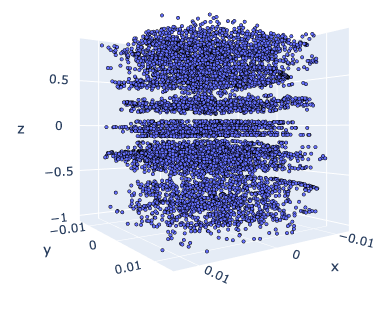
\includegraphics[width=0.49\textwidth, height=6cm, keepaspectratio]{hits_normalised.png}\label{fig:hits_norm}}
\subfloat[Noise Timeslice]{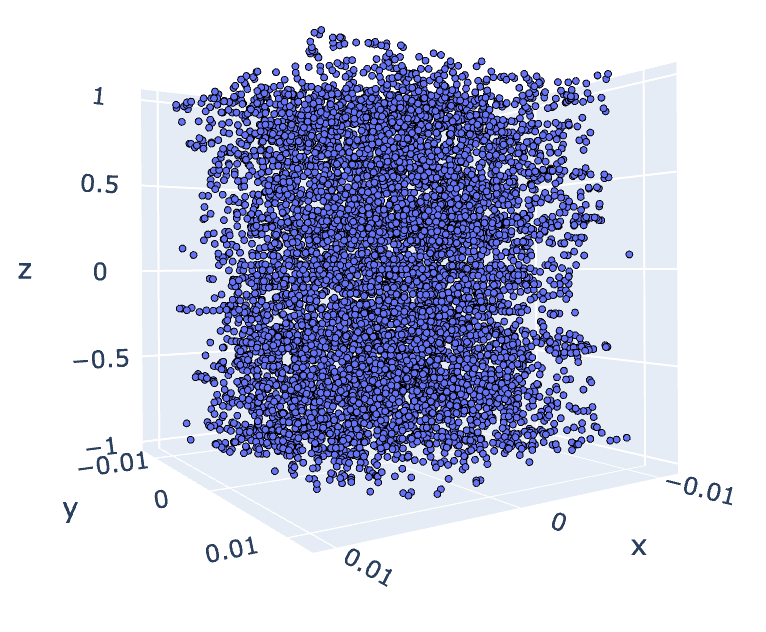
\includegraphics[width=0.49\textwidth, height=6cm,keepaspectratio]{noise_normalised.png}\label{fig:noise_norm}}
\caption[]{An Example of Noise and Events Timeslice After Normalisation}
\label{fig:normalised}
\end{figure}

Point clouds in the KM3NeT dataset have different sizes and are often placed in different parts of the coordinate system. Qi et al. (2017) normalised point clouds along a unit sphere \cite{qi2017pointnet}. The thesis also applied similar translations. Point cloud were translated to the origin by subtracting the mean from all its points, and then normalising them into a unit sphere \cite{qi2017pointnet}. Figure \ref{fig:normalised} shows the effect of this normalisation for both classes.

Qi et al. (2017) also augmented point clouds during training by adding jitter and randomly rotating the objects \cite{qi2017pointnet}. Therefore, the event and noise point clouds were randomly rotated around the Z-axis. Jitter via Gaussian noise was also added with \texttt{0} mean and \texttt{0.02} standard deviation \cite{qi2017pointnet}. Figure \ref{fig:augmented} shows the effect of these augmentations for both classes. 

\begin{figure}[ht!]   
\centering
\subfloat[Event Hits Timeslice]{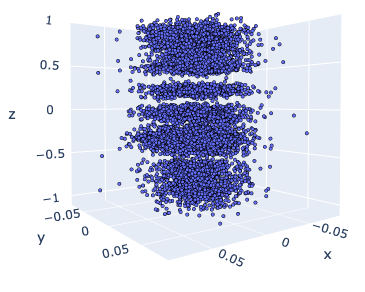
\includegraphics[width=0.49\textwidth, height=6cm, keepaspectratio]{hits_augmented.png}\label{fig:hits_aug}}
\hspace{0.01cm}
\subfloat[Noise Timeslice]{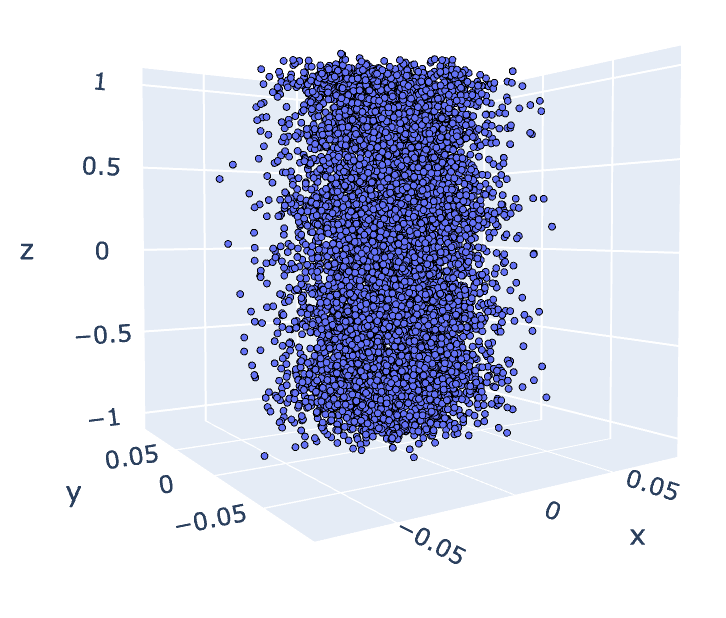
\includegraphics[width=0.49\textwidth,height=6cm, keepaspectratio]{noise_augmented.png}\label{fig:noise_aug}}
\caption[]{An Example of Noise and Event Timeslices After Jitter and Random Rotation}
\label{fig:augmented}
\end{figure}

The application of the recommended augmentations resulted two fairly distinct point clouds and was considered effective. The noise timeslice formed a dense block while the events timeslice formed a collection of points with gaps in between.

Figure \ref{fig:core_pipeline} shows an overview of the pipeline that was used for each of the three datasets - \texttt{(x y time)}, \texttt{(x z time)} and \texttt{(y z time)}. First, 3D coordinates were generated and separated into two classes. Feature engineering using radius-based outlier filter eliminated several points, enhancing event clusters. Surface Poisson Reconstruction was applied to convert the coordinates to 3D meshes. PointNet transformation functions were also added to enhance the point clouds on the fly during training and testing.

\begin{figure}[ht!]
    \centering
    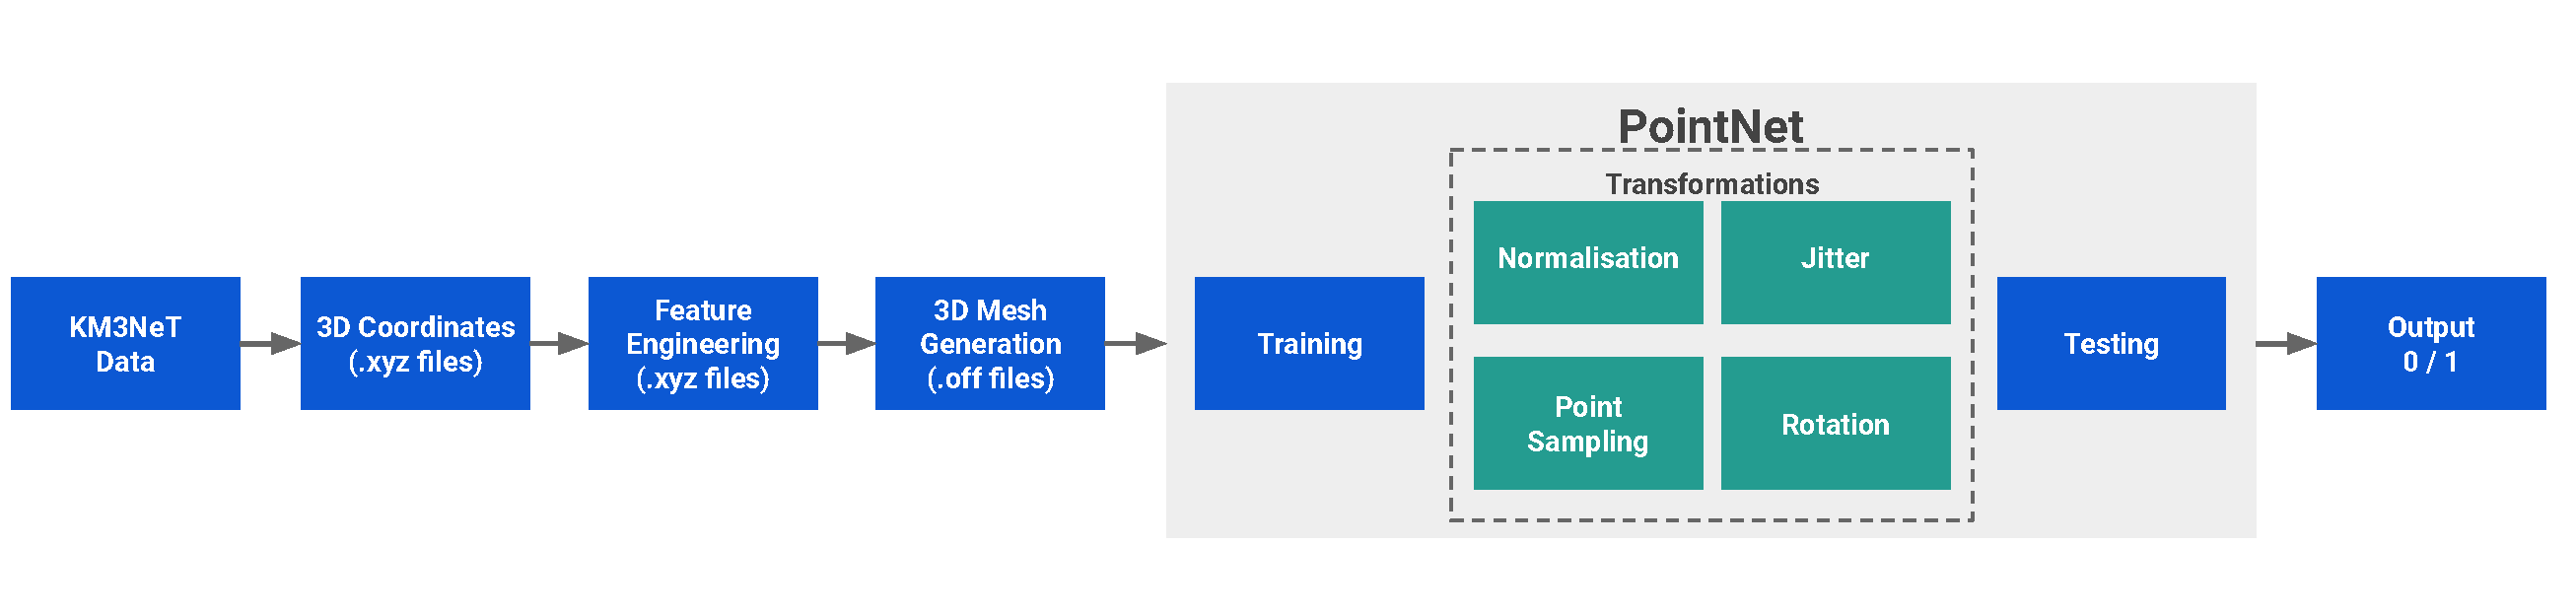
\includegraphics[trim={5.25cm 0 5.5cm 0}, clip, width=\linewidth,keepaspectratio]{core_pipeline}
    \caption{KM3NeT Pipeline Components}
    \label{fig:core_pipeline}
\end{figure}

\let\cleardoublepage\clearpage

